%************************************************
\chapter{Pruebas de Conocimiento Cero}\label{ch:zkp} 
%************************************************

% REF
% Fundamentals
% https://es.wikipedia.org/wiki/Prueba_de_conocimiento_cero
%


% Intro
% Ejemplo intuitivo del laberinto
% Pruebas interacticas: completitud y solvencia/solidez/robustez == completo y robusto/sólido, apartado corto, poner QR en el siguiente
% Prueba de conocimiento cero
%	Perfect vs Comp.
%	QR: es Perfect ZKP, y aplicaciones (id de Shamir, ...)
%	

% TODO: teorema de que el logaritmo discreto tiene un ZKP (para Schnorr). Buscar si existe demostración, por si no es perfect



Las pruebas de conocimiento cero, con siglas ZKP del inglés \textit{Zero-Knowledge Proofs}, permiten demostrar la veracidad de una declaración, sin revelar nada más de ella. En las ZKP intervienen dos partes, el \textit{Prover} y el \textit{Verifier}, o probador y verificador. El prover asegura que una declaración es cierta, y el verifier quiere convencerse de ello a través de una interacción con el prover, de modo que al final de la misma, o bien acaba convencido de que la declaración es cierta, o bien descubre, con una alta probabilidad, que el prover mentía.

Las pruebas de conocimiento cero surgen a partir de los sistemas de pruebas interactivas, que forman una parte importante de la teoría de complejidad computacional, y pidiendo la propiedad de \textit{conocimiento cero} obtenemos el subconjunto de sistemas interactivos que conforman las pruebas de conocimiento cero.

Las referencias para este capítulo se pueden encontrar en %TODO


\section{Una pequeña historia}
%Wikipedia

Antes de estudiar formalmente las ZKP, vamos a ver un ejemplo que se publicó originalmente como un cuento sobre la cueva de Alí Babá \citep{ZKPcave:story}, pero que aquí adaptamos para resumirlo.

\hfil

Imaginemos una cueva donde el camino se bifurca y al final de cada pasillo se juntan ambos caminos formando una especie de anillo. En el punto en que se unen dentro de la cueva, hay una puerta con un código secreto que permite abrirla desde ambos lados, para cruzar al otro pasillo.

\textbf{P}eggy conoce la clave secreta y quiere \textbf{p}robarlo a su amigo Víctor, pero sin tener que revelársela.
\marginpar{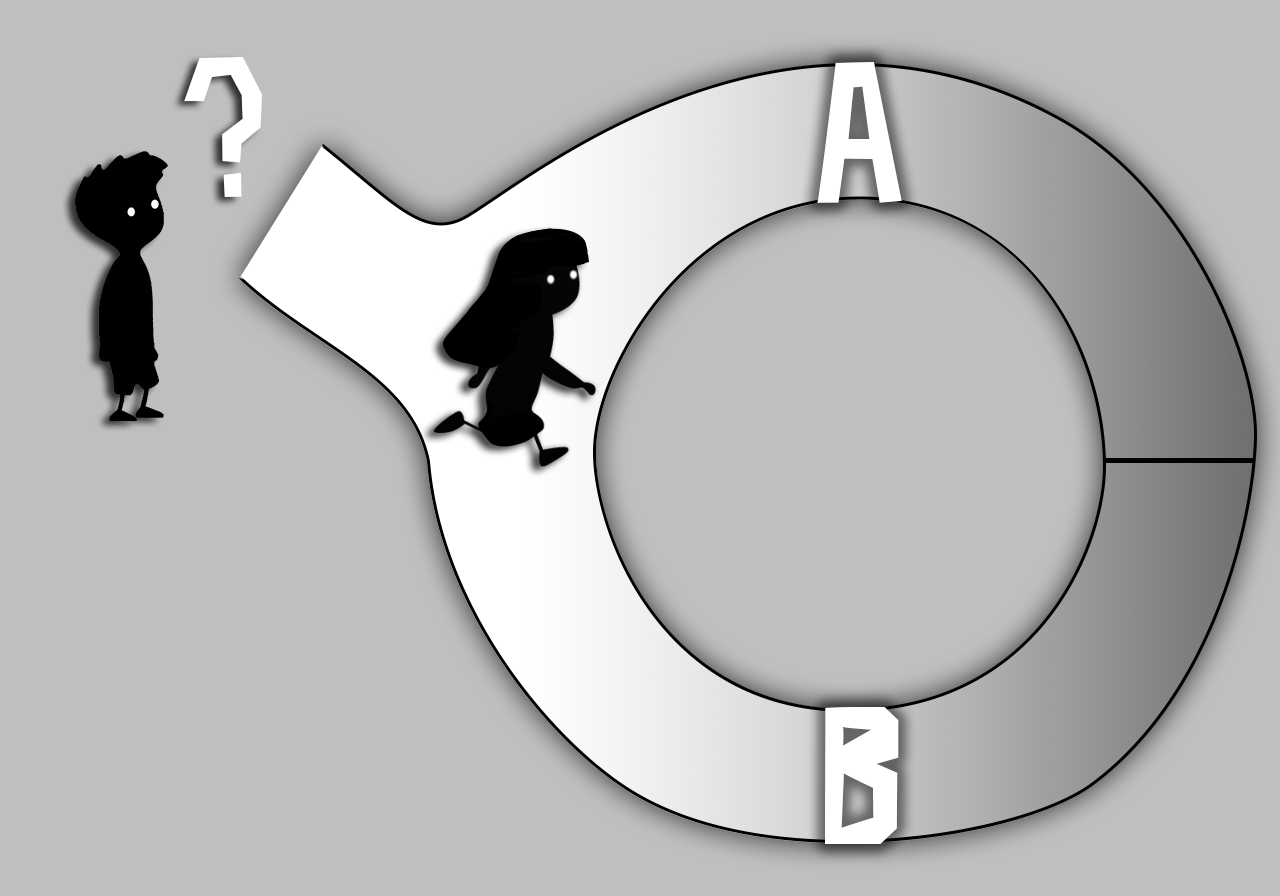
\includegraphics[width=1.\linewidth]{gfx/graficoJL_ZKP_1}\\La cueva \citep{ZKPcave:fig}. Peggy entra por A o B al azar. Víctor espera fuera.}
Peggy y Víctor quedan en la entrada de la cueva con unos \textit{walkie-talkies}, de modo que Víctor esperará fuera y Peggy entrará a la cueva y tomará uno de los pasillos, que llamaremos A y B, sin decirle cuál a Víctor.

%\begin{figure}[bth]
%	\begin{center}
%		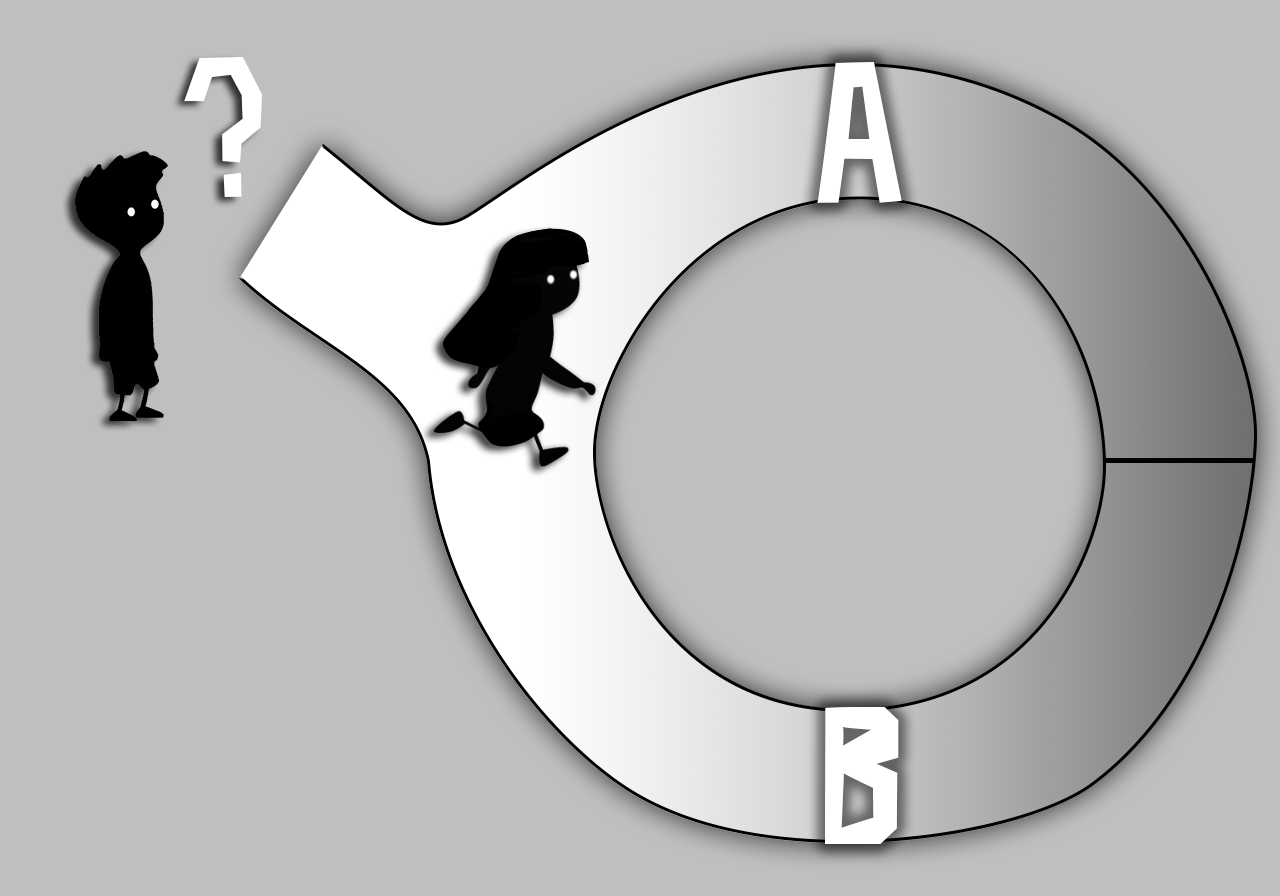
\includegraphics[width=.45\linewidth]{gfx/graficoJL_ZKP_1}
%	\end{center}
%	\caption{La cueva \citep{ZKPcave:fig}. Peggy entra por A o B al azar, Víctor espera fuera.}
%	\label{fig:ZKPcave1}
%\end{figure}

Al llegar a la puerta, avisa a Víctor para que entre a la cueva y espere en la bifurcación, donde \textbf{V}íctor, para intentar \textbf{v}erificar que Peggy conoce la clave, le indicará por qué pasillo quiere que vuelva, el A o el B.


%\begin{figure}[bth]
%	\begin{center}
%		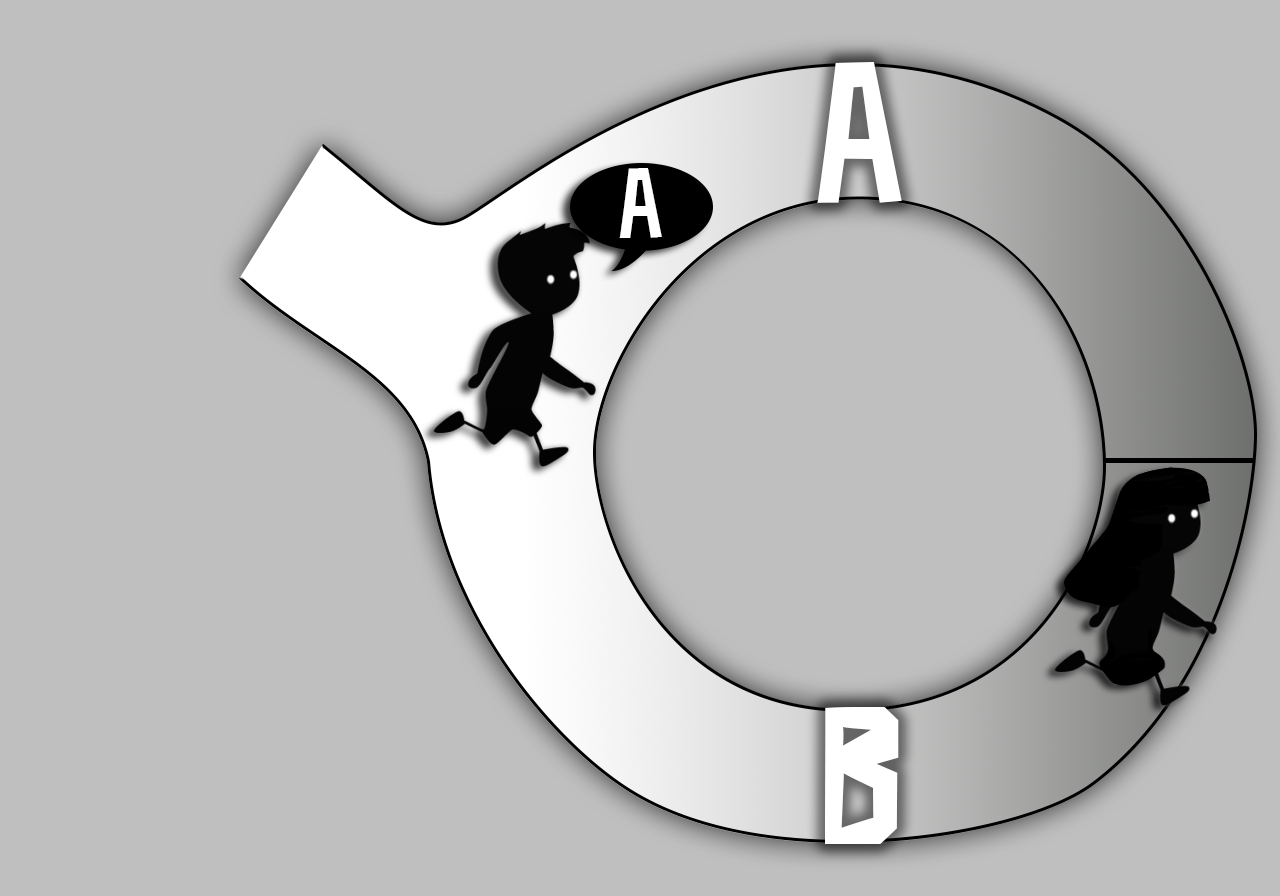
\includegraphics[width=.45\linewidth]{gfx/graficoJL_ZKP_2}
%	\end{center}
%	\caption{La cueva. Víctor elige al azar por dónde quiere que regrese Peggy.}
%	\label{fig:ZKPcave2}
%\end{figure}

Si Peggy realmente conoce la clave, podrá volver a la bifurcación por el pasillo solicitado, abriendo, si es preciso, la puerta.\marginpar{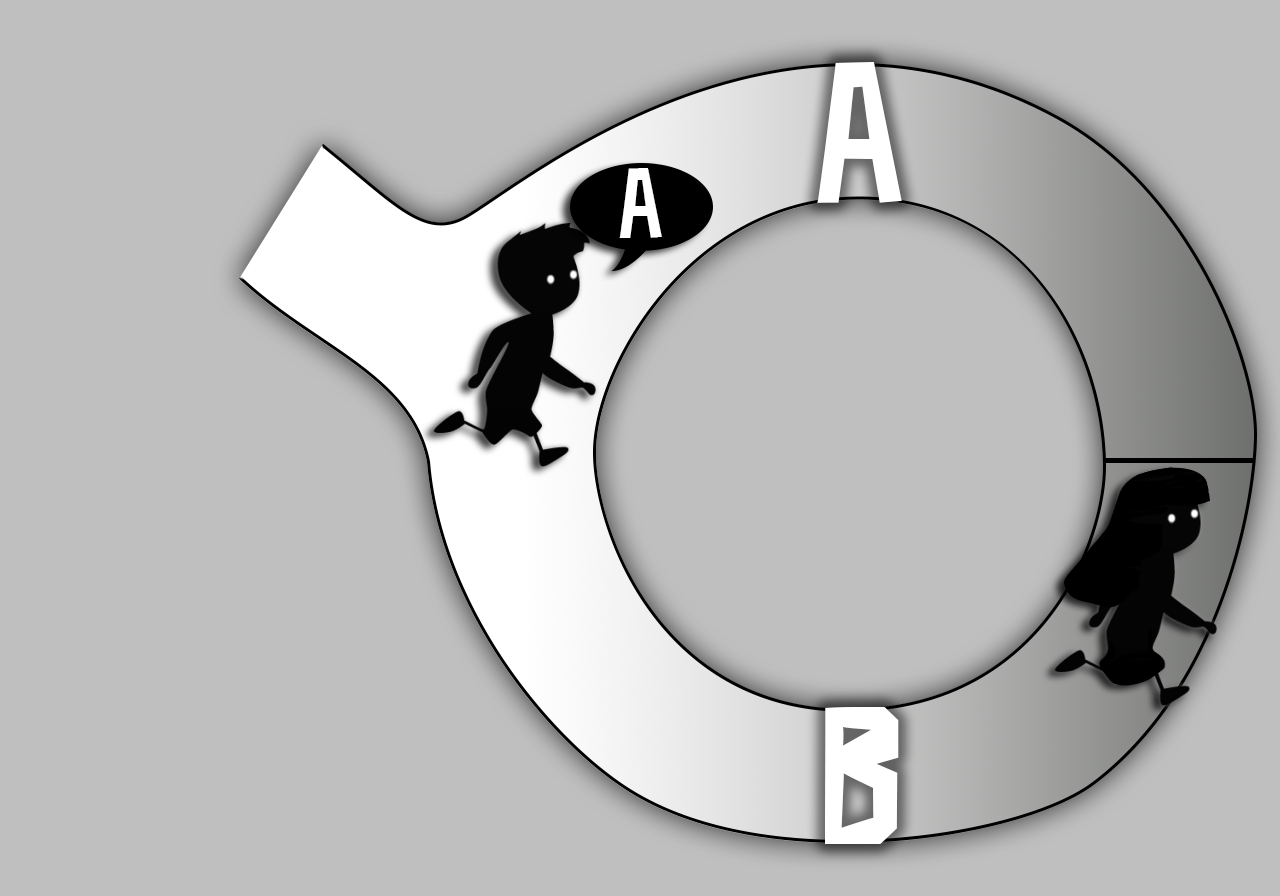
\includegraphics[width=1.\linewidth]{gfx/graficoJL_ZKP_2}\\La cueva. Víctor elige al azar por dónde quiere que regrese Peggy.}
En caso de que no conociera la clave, al entrar tenía una probabilidad del $50\%$ de adivinar qué pasillo pediría Víctor.


%\begin{figure}[bth]
%	\begin{center}
%		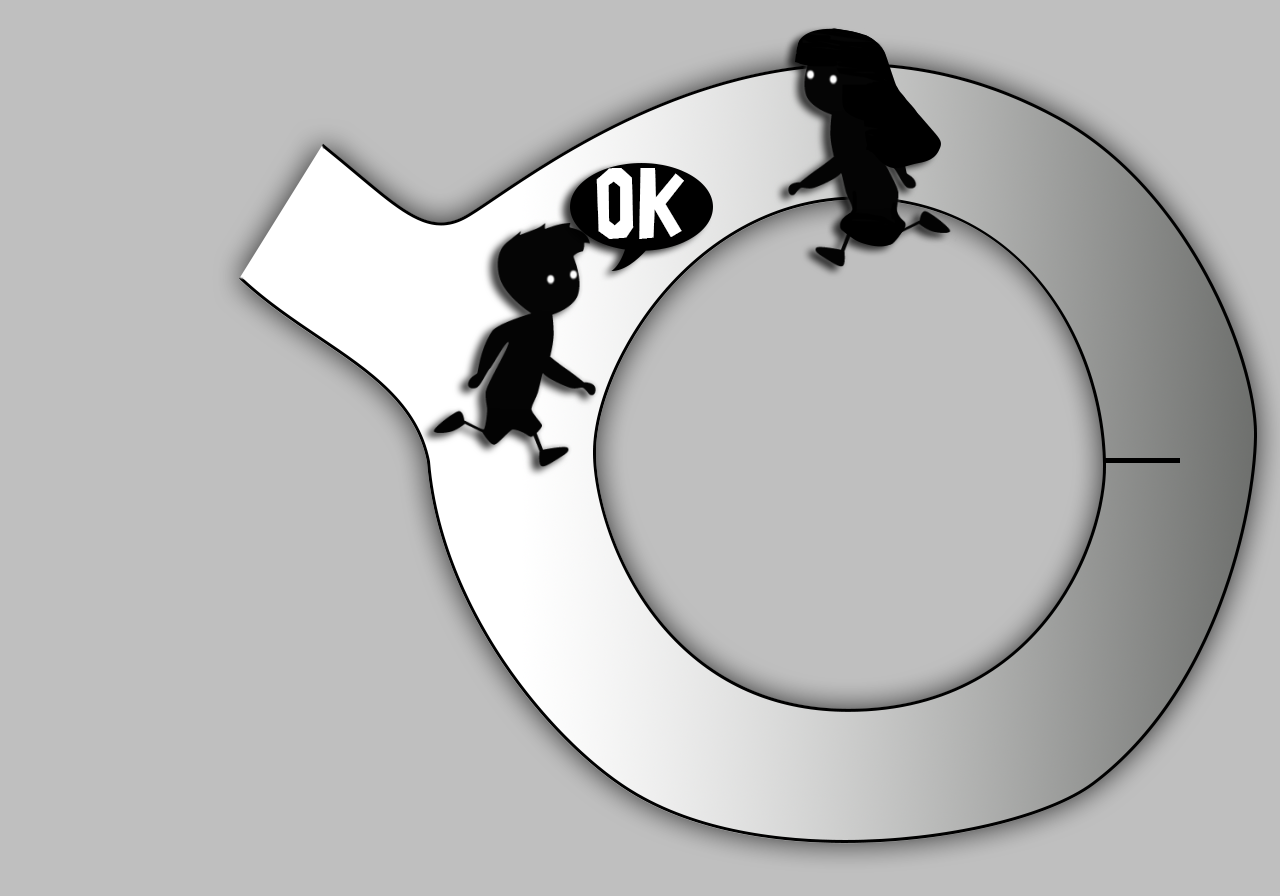
\includegraphics[width=.45\linewidth]{gfx/graficoJL_ZKP_3}
%	\end{center}
%	\caption{La cueva. Peggy vuelve por el camino pedido.}
%	\label{fig:ZKPcave3}
%\end{figure}

Víctor no se queda contento con una sola prueba, así que la repiten hasta que se convence. Si lo repitieran, por ejemplo, 20 veces, Peggy tendría solo una probabilidad de $2^{-20}$, prácticamente nula, de acertar todas las veces y engañar a Víctor.
\marginpar{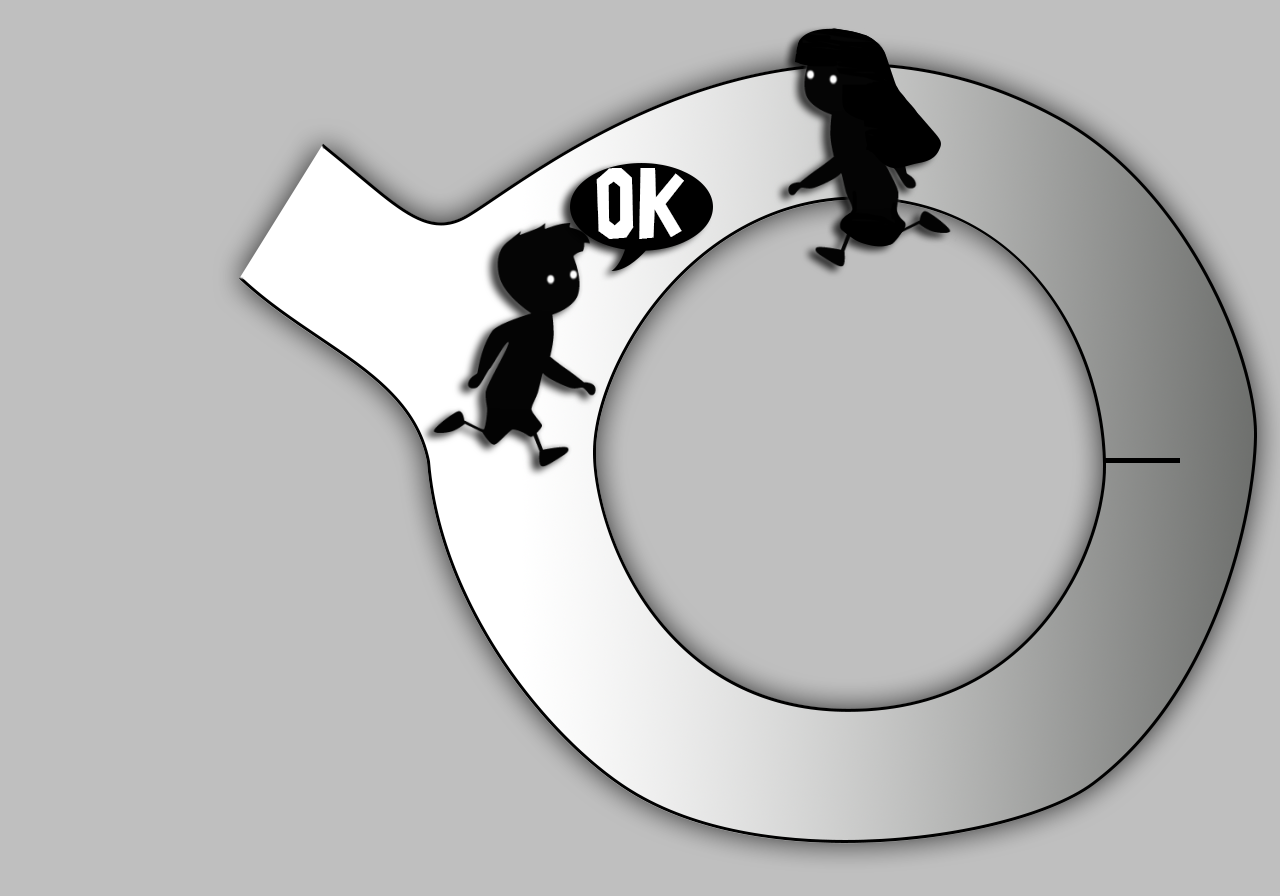
\includegraphics[width=1.\linewidth]{gfx/graficoJL_ZKP_3}\\La cueva. Peggy vuelve por el camino pedido.}


\textbf{E}va, curiosa de qué hacían Víctor y Peggy en la cueva, \textbf{e}spía a Víctor durante todo el proceso. Eva no sabe si Peggy y Víctor han acordado previamente qué pasillo pedir por el \textit{walkie-talkie}, y sólo Víctor está seguro de que los estaba eligiendo al azar, por eso, Eva no puede estar segura de si Peggy conoce la clave secreta, o bien estaban \textbf{s}imulando todo para engañarla por cotilla.

\hfil

\section{Sistemas de Pruebas Interactivas}

\section{Pruebas de conocimiento cero}

\subsection{Pruebas de conocimiento cero perfectas}

\subsection{Pruebas de conocimiento cero estadísticas}

\subsection{Pruebas de conocimiento cero computacionales}


\section{Protocolos de identificación basados en ZKP}
% Puede que para el siguiente capítulo
% Fiat-Shamir, FFS, GQ, Schnorr

